\chapter{Introduction}

%Reachi is a coordinated effort to enable vital communication during emergencies such as natural disasters, where earthquakes, tsunamis, forest fires, and more, destroy the pre-existing communication infrastructure, rendering it near impossible to organise the relief effort to effectively aid the affected, assess the damage, as well as organising repairs to the damaged infrastructure. The goal of the Reachi project is to optimise the disaster response by creating an overview of the situation within the first eight hours after the disaster. Today, this process can take up 1-2 weeks, due to the destruction of pre-existing communication infrastructure~\cite{website:reachiproject}. Without this overview, it is impossible to know where the needs for disaster relief is greatest, or what the level of disaster relief is even available. The project has been developed by the danish company LinkAiders ApS, and utilise a technology to enable mobile ad-hoc mesh networking through radio communication, created by NeoCortec.

%\begin{figure}[H]
%    \centering
%    \begin{subfigure}[]{.2\textwidth}
%        \qrcode[hyperlink,height=1.0in]{https://www.youtube.com/watch?v=Hh2Cw6GhBRU}
%        %\caption{2000 nodes.}
%        \label{figure:clustering:2knodes}
%    \end{subfigure}
%    \begin{subfigure}[]{.79\textwidth}
%        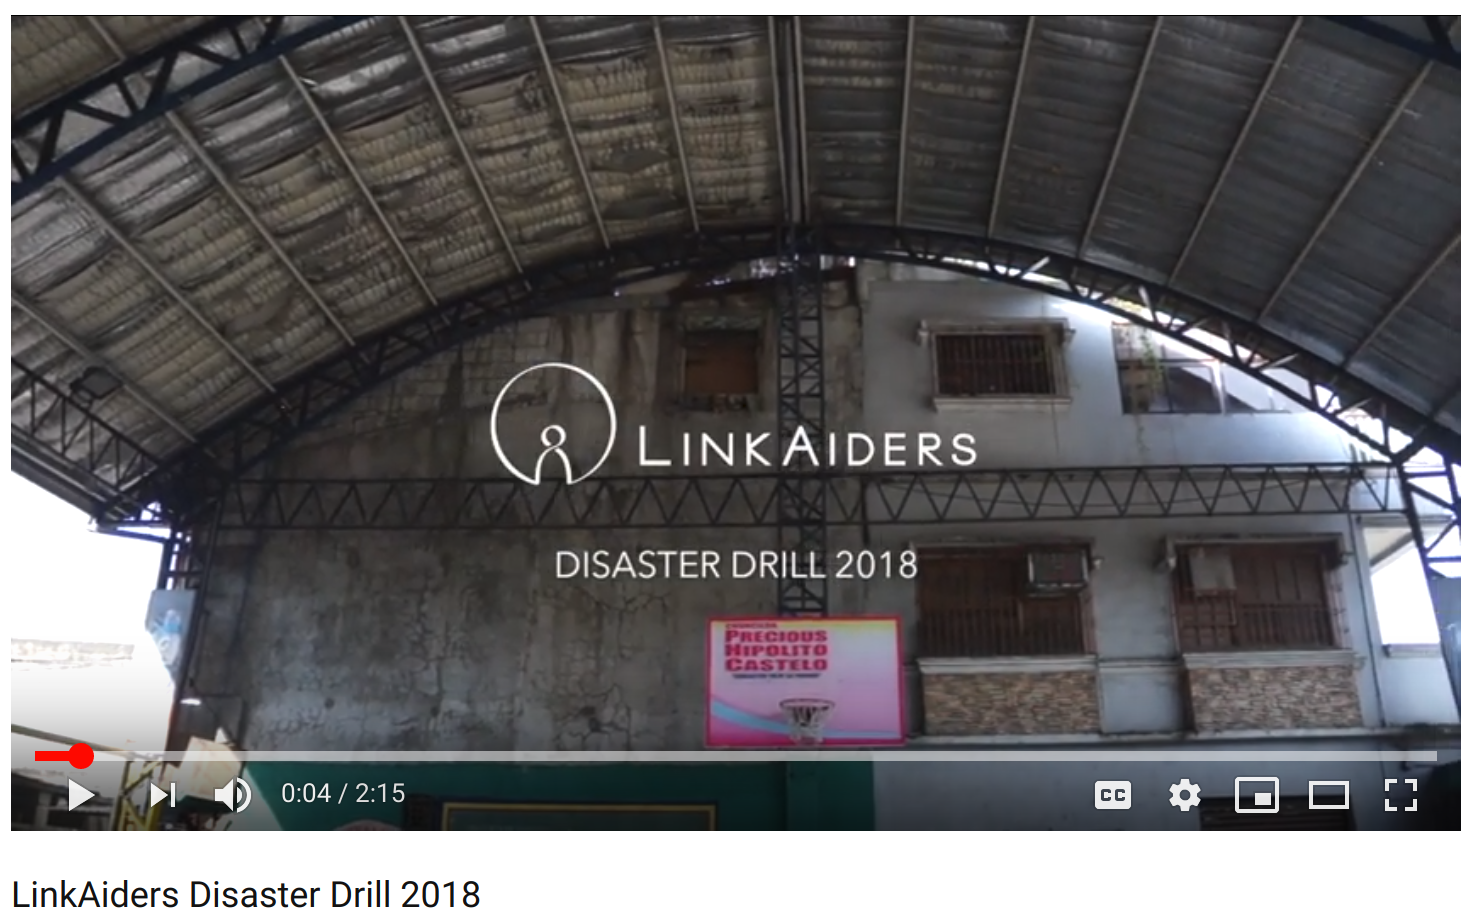
\includegraphics[width=\linewidth]{figures/linkaiders-drill-320.png}
%        %\caption{2000 nodes clustered.}
%        \label{figure:clustering:2k80m2ptsnodes}
%    \end{subfigure}
%    \caption{A YouTube video, showing the largest scale drill of the Reachi project with 320 volunteers.}
%    \label{figure:introduction:reachi-test}
%\end{figure}

%To date, the largest scale drill of the Reachi system was conducted in September 2018, in the Phillippines, with the help of 320 volunteers. The drill was conducted in order to test the Reachi system as a needs assessment tool, the volunteers' ability to use the Reachi devices, as well as the ability of the Reachi system to create the necessary overview of the situation, in less than eight hours. A video of the drill has been uploaded to the LinkAiders ApS YouTube channel, and the link is encoded in the QR Code in \autoref{figure:introduction:reachi-test}. \medbreak

%The goal for the Reachi project is to scale, and test, the project with up to 1000 devices~\cite{website:reachiproject}, which is a massive undertaking, and would require even more effort to organise such a drill. Our project proposes a C++ library for writing, and running, simulations of the network protocol behind the mesh communication in a \gls{manet}, using state-of-the-art modelling of link \gls{pathloss} behind the radio communication, to simulate packet loss and collisions caused by interference. With our library, it would be possible to write a C++ implementation of communication protocols, such as \gls{lmac}~\cite{paper:lmac_protocol} or Slotted ALOHA~\cite{Roberts:1975:APS:1024916.1024920}, using a simple interface header file resembling a traditional hardware interface.

% https://www.youtube.com/watch?v=Hh2Cw6GhBRU

% https://markedsmodningsfonden.dk/reachi-vital-informationsdeling-i-katastrofesituationer

% - motivation / aim
% - Why do the project?
%Verifying that \gls{manet} protocols work as intended, is essential if the protocol is to be used in a real world setting, especially in critically important settings. Testing a \gls{manet} protocol with many nodes and emulating the setting the protocol will be used in can be problematic, as the setting might be hard to recreate in a way that makes the collection of data possible or creating a large enough network.\medbreak
% tickle some more
% - Run the actual software, in a realistic setting


%This gives reason to develop a framework, capable of simulating arbitrary \gls{manet} protocols. Designing the framework to run on a cluster will allow for the usage of \gls{mpi}, thus increasing the possible scale and speed of the simulation.
%Since the protocols are of the wireless nature, we need a way to simulate the probability of loosing a packet or the packet containing errors. In other words calculating the \gls{pep}.

%At the time of writing, there exists several well-established \gls{mpi} implementations for several languages. Our framework will utilise one of those well-established implementations and add a layer on top of that, where the \gls{pep} calculations will happen.

%Lastly we will test the framework on an \gls{manet} protocol, on the cluster available at Aalborg University, to verify that the framework works on a real world protocol.